\documentclass{article}

% Packages
\usepackage[utf8]{inputenc}
\usepackage{hyperref}
\usepackage{graphics}
\usepackage{graphicx}
\usepackage{caption}
\usepackage{minted}
\usepackage{datetime}
\usepackage{amsmath}
\usepackage[
    backend=bibtex,
    style=numeric,
    bibencoding=ascii,
    sorting=ynt
]{biblatex}

% Bibliography linking
\addbibresource{resources}

% Configuration for packages
\renewcommand*\contentsname{Tabelă de Conținut}
\renewcommand{\listtablename}{Listă de Tabele}
\renewcommand*\listfigurename{Listă de Imagini}
\captionsetup[table]{name=Tabel}
\renewcommand*\figurename{Imagine}
\usemintedstyle{bw}
\hyphenpenalty=100000

% Content of title page
\title{
    
\includegraphics[width=3cm, height=3.5cm]{images/ATM.png} \\
    \vspace{5mm}
    Descrierea Aplicației \textbf{Naevia}
    \vspace{10mm}
}
\vspace{20mm}
\author{
    Apostolescu Ștefan \\
    Băjan Ionuț-Mihăiță \\
    Iosif George-Andrei \\
    \vspace{10mm}
}
\ddmmyyyydate

% Beginning of the document
\begin{document}

% Title page
\null
\nointerlineskip 
\vfill
\let\snewpage \newpage
\let\newpage \relax
\clearpage\maketitle
\thispagestyle{empty}
\let \newpage \snewpage
\vfill 
\break

\newpage

% Table of content
\setcounter{page}{1}
\tableofcontents

\newpage

% Section
\section{Introducere}

Aplicația dezvoltată ca temă pentru cursul de "\textit{Inteligență Artificială}" poartă numele de \textbf{Naevia}. Aceasta își propune folosirea tehnicii \textit{Hill Climbing} pentru optimizarea procesului de criptanaliza a unor cifruri clasice. În același timp, prin intermediul ei, se pot cripta texte cu ajutorul cifrurilor implementate și face comparații între abordarea bazată pe forță brută (engl. "\textit{brute-force}") și cea optimizată, prin intermediul unui grafic ce ilustrează dificultatea cu care o anumită abordare tinde spre o soluție. 

De menționat este principalul dezavantaj al folosirii \textit{Hill Climbing} pentru criptanaliză. Acesta constă în faptul că tehnica asigură numai găsirea unei soluții locale, care poate coincide cu textul în clar inițial, folosit în procesul de criptare. Din acest motiv, pentru cazurile în care soluția returnată nu este cea validă (lucru determinat, de exemplu, prin intermediul sensului avut de text) se recomandă rularea repetată pentru că, la fiecare rulare, punctul de plecare din spațiul de valori (în cazul de față, cheia încercată în procesul de decriptare) este unul diferit.

% Section
\section{Noțiuni Teoretice}

\subsection{Cifruri Clasice}

\subsubsection{Caesar}

Cifrul lui Caesar este un sistem de cifrare monoalfabetic pentru care textul în clar este construit din literele alfabetului latin (de la A la Z) și din cheia de cifrare, reprezentată de un număr întreg k $ \in $  $ \{ $ 0, ..., 25$ \} $.

\vspace{0.3cm}
\begin{center}
    \fbox{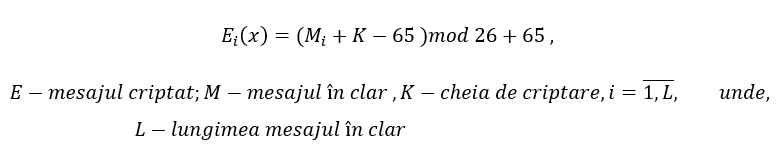
\includegraphics[width=10cm]{images/equations/4.png}}
    \label{fig:1}
    \captionsetup{justification=centering,margin=1cm}
    \captionof{figure}{Criptarea unui text cu ajutorul cifrului Caesar}
\end{center}
\vspace{0.3cm}

\begin{center}
    \fbox{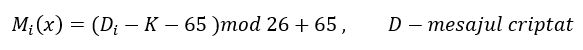
\includegraphics[width=7cm]{images/equations/5.png}}
    \label{fig:2}
    \captionsetup{justification=centering,margin=1cm}
    \captionof{figure}{Decriptarea unui text cu ajutorul cifrului Caesar}
\end{center}
\vspace{0.3cm}

\begin{center}
    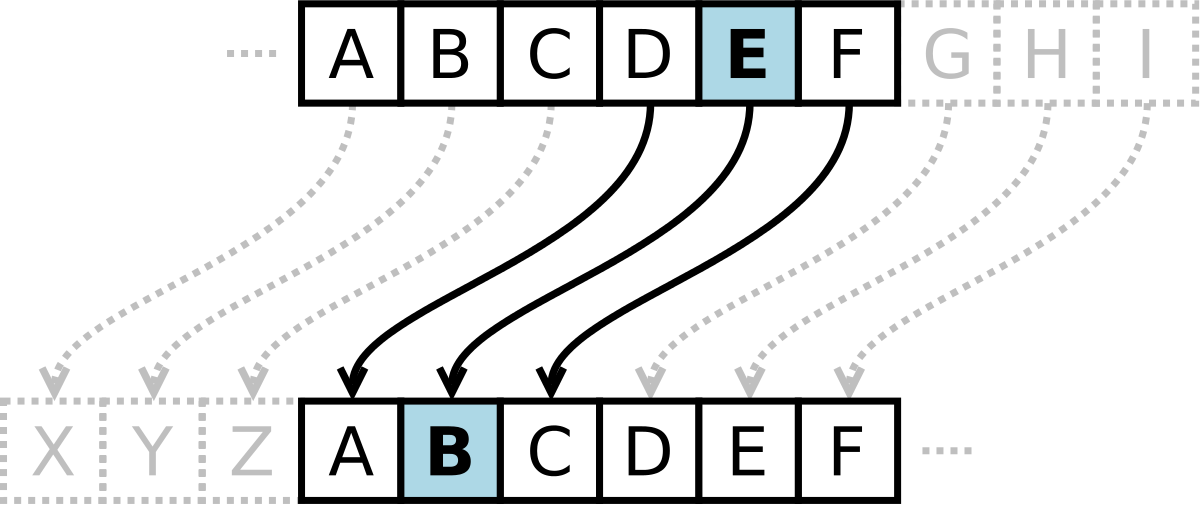
\includegraphics[width=7cm]{images/caesar.png}
    \label{fig:2}
    \captionsetup{justification=centering,margin=1cm}
    \captionof{figure}{Transformarea alfabetului în cadrul cifrului Caesar}
\end{center}
\vspace{0.3cm}

După cum se observă, acest cifru este unul simplu întrucât, în procesul de criptare, fiecare caracter din mesajul inițial este deplasat circular în cadrul alfabetului. În acest sens, complexitatea algoritului de cifrare este direct proporțională cu lungimea alfabetului. În cazul alfabetului în limba engleză, sunt necesare 26 de încercări, folosind un atac cu forță brută, pentru a afla mesajul inițial.

\subsubsection{Vigenère}

Cifrul lui Vigenère este o metodă de criptare care folosește o serie de cifruri Caesar diferite, bazate pe literele unui cuvânt-cheie. Este o formă simplă de substituție polialfabetică. În acest cifru, cheia de criptare este reprezentată de o parolă (de regulă, un cuvânt). Dacă dimensiunea cheii de criptare este mai mică decât cea a mesajului, se repetă cheia până la finalizarea codificării mesajului.

\vspace{0.3cm}
\begin{center}
    \fbox{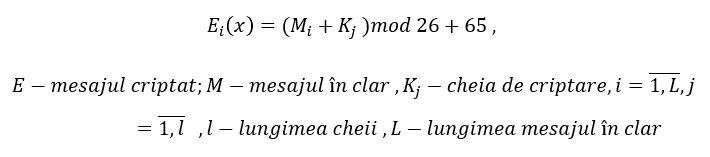
\includegraphics[width=10cm]{images/equations/6.png}}
    \label{fig:2}
    \captionsetup{justification=centering,margin=1cm}
    \captionof{figure}{Criptarea unui text cu ajutorul cifrului Vigenère}
\end{center}
\vspace{0.3cm}

\begin{center}
    \fbox{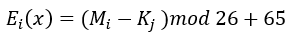
\includegraphics[width=4cm]{images/equations/7.png}}
    \label{fig:2}
    \captionsetup{justification=centering,margin=1cm}
    \captionof{figure}{Decriptarea unui text cu ajutorul cifrului Vigenère}
\end{center}
\vspace{0.3cm}

Complexitatea acestui cifru este dată de lungimea cheii folosite. Presupând că un atacator ghicește lungimea parolei, spargerea cifrului Vigenère poate fi tratată ca în cazul cifrului Caesar. Pentru a afla lungimea chei se pot folosi următoarele teste:
\begin{itemize}
    \item Kasiski, ce profită de faptul că toate cuvintele repetate sunt, din întâmplare, uneori criptate folosind aceleași litere-cheie, ceea ce duce la grupuri repetate în textul cifrat; și
    \item Friedman, ce se bazează pe indicele de coincidență, care măsoară denivelarea frecvențelor literelor cifrate pentru a sparge cifrul.
\end{itemize}

\subsubsection{De Substituție}

Operația de criptare în cadrul cifrului de substituție se bazează pe o corespondență biunivocă între alfabetul clar și cel cifrat. Cheia de criptare în acest cifru este reprezentată de o permutare a dicționarului folosit la generarea mesajului inițial. Permutarea poate fi aleatoare sau pseudoaleatoare.

\vspace{0.3cm}
\begin{center}
    \fbox{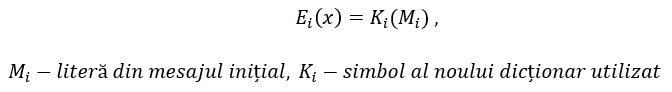
\includegraphics[width=10cm]{images/equations/8.png}}
    \label{fig:2}
    \captionsetup{justification=centering,margin=1cm}
    \captionof{figure}{Criptarea unui text cu ajutorul cifrului de substituție}
\end{center}
\vspace{0.3cm}

\begin{center}
    \fbox{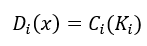
\includegraphics[width=3cm]{images/equations/9.png}}
    \label{fig:2}
    \captionsetup{justification=centering,margin=1cm}
    \captionof{figure}{Decriptarea unui text cu ajutorul cifrului de substituție}
\end{center}
\vspace{0.3cm}

La o primă vedere, pentru spargerea acestui cifru printr-un atac prin forță brută, avem un spațiu total al tutoror cheilor posibile de aproximativ 26 factorial (număr reprezentat pe aproximativ 88 de biți). Însă de considerat este faptul că, în practică, ultimele litere ale alfabetului (care sunt în mare parte de frecvență joasă) tind să rămână la sfârșit. Acest lucru reduce semnificativ timpul de spargere a cheii de criptare.

\subsection{\textit{Hill Climbing}}

\textit{Hill Climbing} este un algoritm de căutare optimizată a soluțiilor unei probleme care se poate rezolva prin minimizare. Acesta folosește o funcție de euristică, precum și o funcție de generare de stări, amândouă specifice fiecărei probleme în parte. Algoritmul pornește de la o stare inițială și, prin iterații succesive, ajunge la un punct de minim local.

\newpage

\section{Folosirea \textit{Hill Climbing} în Contextul Criptanalizei}

\textit{Hill Climbing} poate fi aplicat în cripanaliza clasică, bazată pe substituție, pentru spargerea cheii de criptare. 

Algoritmul pleacă de la o cheie inițială, dată sau alesă aleator. Cu ajutorul funcției de generare de stări, se derivă o mulțime de alte chei. Textul este decriptat cu ajutorul acestor chei și, pentru fiecare variantă a textului decriptat, se calculează o metrică. Din mulțimea de chei generate anterior se alege cheia pentru care textul decriptat are euristica (metrica stabilită) cea mai mică. Euristica este calculată în așa fel încât să tindă spre 0 atunci când textul decriptat este în limba engleză.

Procesele de derivare, decriptare și de calculare a euristicii se repetă până când nu se mai găsește o cheie cu euristică mai mică decât cheia curentă.

\subsection{Funcția de Generare de Stări}

În cazul criptografiei clasice, bazată pe substituție, funcția de generare de stări reprezintă funcția de derivare de chei. Aceasta primește ca parametru o cheie inițială și returnează o mulțime de chei derivate din aceasta. Cheile derivate sunt obținute aplicând permutări literelor cheii inițiale, cât și înlocuind aleator litere acesteia. Mulțimea obținută conține chei unice atât la nivel local (toate cheile generate într-o iterație) cât și la nivel global (toate cheile deja generate).

\subsection{Funcția Euristică}

Funcția euristică își propune să determine asemănarea textului descifrat cu unul în limba engleză. Aceasta se poate verifica numărând frecvența de apariție a literelor sau a grupurilor de litere din textul decriptat și comparând frecvențele cu cele determinate empiric, ale limbii engleze. Cu cât textul se apropie de unul în limba engleză, cu atât mai mult va scădea valoarea euristicii.

\vspace{0.3cm}
\begin{center}
    \fbox{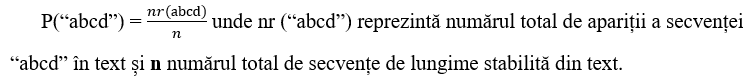
\includegraphics[width=10cm]{images/equations/1.png}}
    \label{fig:1}
    \captionsetup{justification=centering,margin=1cm}
    \captionof{figure}{Formula pentru calcularea frecvenței unei grupări de 4 litere}
\end{center}
\vspace{0.3cm}

\begin{center}
    \fbox{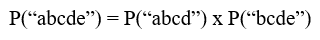
\includegraphics[width=5cm]{images/equations/2.png}}
    \label{fig:1}
    \captionsetup{justification=centering,margin=1cm}
    \captionof{figure}{Formula pentru calcularea frecvenței unei grupări de 5 litere}
\end{center}
\vspace{0.3cm}

Pentru un text de lungime medie, calculul tuturor frecvențelor va presupune multe înmulțiri și vor apărea erori numerice de calcul. Pentru a evita acest lucru, se va calcula logaritmul fiecărei probabilități astfel:

\vspace{0.3cm}
\begin{center}
    \fbox{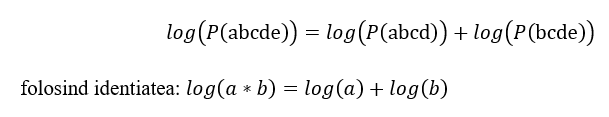
\includegraphics[width=10cm]{images/equations/3.png}}
\end{center}
\vspace{0.3cm}

Practic, calcularea euristicii pentru un text se rezumă la calcularea sumei logaritmilor frecvențelor de apariție a grupurilor de \textit{n} litere, unde \textit{n} este număr natural mai mare decât 1. Pentru aplicația dezvoltată, valoarea lui \textit{n} este egală cu 4.

Dat fiind spațiul uriaș de căutare în cazul substituției pentru o cheie de 26 de caractere, anume $26^{26}$, există o probabilitate mare ca algoritmul să nu găsească din prima iterație minimul global, ci să se oprească la un minim local. De aceea este recomandată rularea de mai multe ori a algoritmului (și folosirea cheii găsite cel mai des) sau analiza manuală a textului decriptat. 

Prin metode experimentale, s-a estimat probabilitatea de găsirii a cheii corecte ca fiind $\frac{2}{3}$ din numărul total de încercări. Această probabilitate variază în funcție de lungimea textului criptat. Cu cat acesta este mai lung, cu atat mai mult vor varia euristicile pentru diferitele chei, iar cheia corectă va fi găsită mai ușor.

% Section
\section{Arhitectura Aplicației}

\vspace{0.3cm}
\begin{center}
    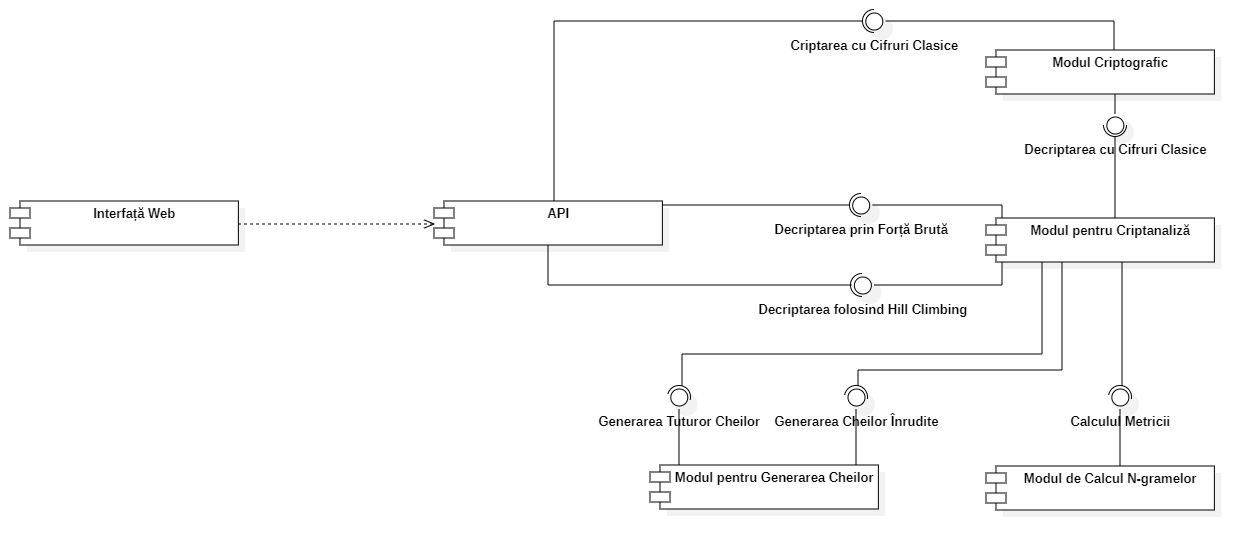
\includegraphics[width=12.5cm]{images/components_diagram.png}
    \label{fig:1}
    \captionsetup{justification=centering,margin=1cm}
    \captionof{figure}{Diagrama de Componente a Aplicației}
\end{center}
\vspace{0.3cm}

% Section
\section{Modul de Utilizare al Aplicației}

Utilizatorii aplicației pot interacționa cu aceasta prin intermediul unei interfețe web, compusă dintr-o singură pagină (engl. "\textit{single-page application}") în care conținutul computațiilor efectuate de serverul web sunt incluse în manieră dinamică în ea, fără a fi necesară o reîncărcare completă.

O interacțiune uzuală cu aplicația conține următorii pași:
\begin{itemize}
    \item accesarea aplicației cu ajutorul unui \textit{browser} web;
    \item selectarea operațiunii ce se dorește efectuată (criptare sau decriptare);
    \item în cazul în care criptarea este aleasă: 
        \begin{itemize}
            \item setarea textului în clar;
            \item alegerea unui cifru disponibil (Caesar, Vigenère sau cifru de substituție);
            \item setarea parolei pentru cifru (un număr pentru Caesar, un șir de caractere pentru Vigenère sau o permutare a alfabetului pentru cifrul de substituție);
            \item apăsarea butonului de trimitere a cererii de criptare;
            \item așteptarea primirii unui răspuns de la serverul web; și
            \item preluarea textului criptat din câmpul specific.
        \end{itemize}
    \item în cazul în care decriptarea este aleasă: 
        \begin{itemize}
            \item setarea textului criptat;
            \item alegerea unui abordări disponibile pentru decriptare (prin \textit{brute-force} sau cu ajutorul tehnicii de optimizare \textit{Hill Climbing});
            \item apăsarea butonului de trimitere a cererii de decriptare;
            \item așteptarea primisii unui răspuns de la serverul web;
            \item preluarea textului decriptat din câmpul specific; și
            \item observarea în grafic a modului în care funcția euristică a tins către soluția returnată.
        \end{itemize}
\end{itemize}

% Section
\section{Concluzii}

În concluzie, aplicația dezvoltată dovedește faptul că tehnica de optimizare \textit{Hill Climbing} poate fi utilizată cu succes în procesul de criptanaliza a unor cifruri clasice. Deși tehnica asigură numai un minim local, deci numai un text care ar putea fi cel inițial, experimentele realizate au demonstrat o eficiență ridicată.

\end{document}